\documentclass[a4paper,12pt]{extarticle}
%\usepackage[T2A]{fontenc}
\usepackage[utf8]{inputenc}
\usepackage[english,russian]{babel}

\usepackage{csquotes}
\usepackage{graphicx}
\usepackage{lmodern}
\usepackage[hidelinks]{hyperref}

\usepackage[style=gost-authoryear,language=auto,backend=biber]{biblatex}
%\usepackage[style=gost-numeric,language=auto,backend=biber]{biblatex}
\addbibresource{Bibliography.bib}
%Настройки вида страниц
\usepackage[left=3cm,right=1.5cm,top=2cm,bottom=2cm,bindingoffset=0cm]{geometry}
\renewcommand{\baselinestretch}{1.5} 

%\makeatletter
%\renewcommand{\@biblabel}[1]{#1.}
%\makeatother

\begin{document}
%\nocite{*}
%Настройка шрифтов 

\fontfamily{cmr}

\begin{titlepage}
\begin{center}
Федеральное Государственное Бюджетное Образовательное Учреждение \\ Высшего Профессионального Образования \\«Московский Государственный Технический Университет имени Н.Э. Баумана» (МГТУ им. Н.Э. Баумана)
\end{center} 
\vfill
{\large \begin{center}
{\Large Реферат} \\по курсу 
"Цифровая обработка сигналов" \\
на тему 
 "Криптографические и стеганографические методы\\ формирования
 и легитимного определения электронной подписи"
\end{center}}
\vfill
\begin{flushright}
Студент Жучков А.\\
  Группа РК6–112\\
Преподаватель Волосатова Т.М.
\end{flushright}
\vfill
\centering Москва 2015
\end{titlepage}
\section{Введение}
\par \hspace{1.25cm}Рукописная подпись используется для удостоверение подлинности
 документа, а также авторства или согласия с содержимым. С масштабным переходом
  к системам электронного документооборота (СЭД), остро встала проблемы
   проверки аутентичности данных и установления авторства электронного
    документа. Для решения данных проблем были разработаны методы электронной подписи документов. Электронная цифровая подпись (ЭЦП) --- особый атрибут электронного документа, хранящийся вмести с ним. Данный атрибут позволяет защитить данные от изменения и однозначно устанавливает связь межу электронной подписью и лицом (группой лиц), подписавшим данный документ.
\par Для мультимедиа файлов, охраняемых авторским правом, также актуальны
 проблемы целостности и аутентификации автора при их передаче, но
  появляется дополнительная задача – пресечение попыток незаконного
   распространения. Данная задача решается, созданием устойчивой электронной
    подписи. Устойчивая ЭЦП (устойчивый водяной знак) -- атрибут мультимедиа файла, хранящий информацию о субъекте авторского права, который нельзя уничтожить обычными манипуляциями с данными. 
\par Такая задача, как определение целостности (подлинности) документов, в
 настоящее время поднимается всё чаще. Это вызвано увеличением объёма документооборота между организациями, а также развитием технологий обмена документами. В связи с этим появляется множество различных методов защиты документов от подделки. Так, возможно применение криптографических методов цифровой подписи (ЭЦП), стойкость которой основывается на сложности вычисления дискретного логарифма в группе точек эллиптической кривой, а также на стойкости хэш-функции \cite{gost34.10}, или стеганографических методов \cite{gupta2015} – встраивания ЦП в электронный документ (изображение) или встраивания ЦВЗ, а также внесения специального шума. 
\section{Методы формирования электронной подписи}
\subsection{Криптографические ЭЦП}
\par Криптографические методы шифрования основаны на использовании хэш-функций и симметричных или асимметричных алгоритмах шифрования. Для подписи электронного документа, на исходном файла вычисляется значение хэш-функции. Затем, хэш шифруется одним из алгоритмов шифорования. Шифрованный хэш используется как ЭЦП и передается получателю вместе с исходным документом. Для защиты сообщения от подмены, подпись передается в специальном контейнере. Схема контейнера представлена на \ref{fig:CryptoPackage}. В контейнере хранится уникальный идентификатор отправителя – ссылку на сертификат. Сертификат содержит идентификатор, свой статус (действителен или отозван) и о способе проверки подлинности ЭЦП. Сертификаты различаются по способу организации их выдачи. Очевидно, что сертификат должен быть выдан некоторым агентом, которому можно доверять. Исторически сложились две системы управления сертификатами: с помощью центров сертификации (стандарт X.509) и на основе сетей доверия (PGP) \cite{polynskay2007}.
\begin{figure}[ht]
\centering
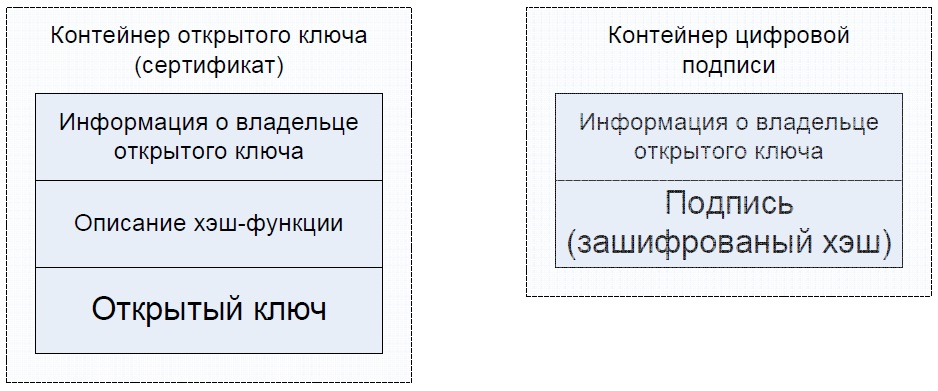
\includegraphics[width=0.7\linewidth]{CryptoPackage}
\caption{Схема контейнера ЭЦП, передаваемого вместе с сообщением.}
\label{fig:CryptoPackage}
\end{figure}
\par Таким образом, данная схема ЭЦП, включает следующие действия. Сторона А для документа вычисляет хеш-функцию, затем полученное значение шифруется с помощью закрытого ключа (private key) получая ЭЦП. Сторона Б получает документ, ЭЦП и сертификат (ссылку на сертификат) стороны А, верифицирует сертификат открытого ключа стороны А в удостоверяющем центре, дешифрует полученную ЭЦП при помощи общего ключа (public key), вычисляет хеш-функцию документа и проверяет с расшифрованым значением. Если сертификат стороны А действителен и проверка прошла успешно, принимается, что документ был подписан стороной А. Данная схема формирования и проверки подписи представлена на \ref{fig:CryptoSchema}.
\begin{figure}[ht]
\centering
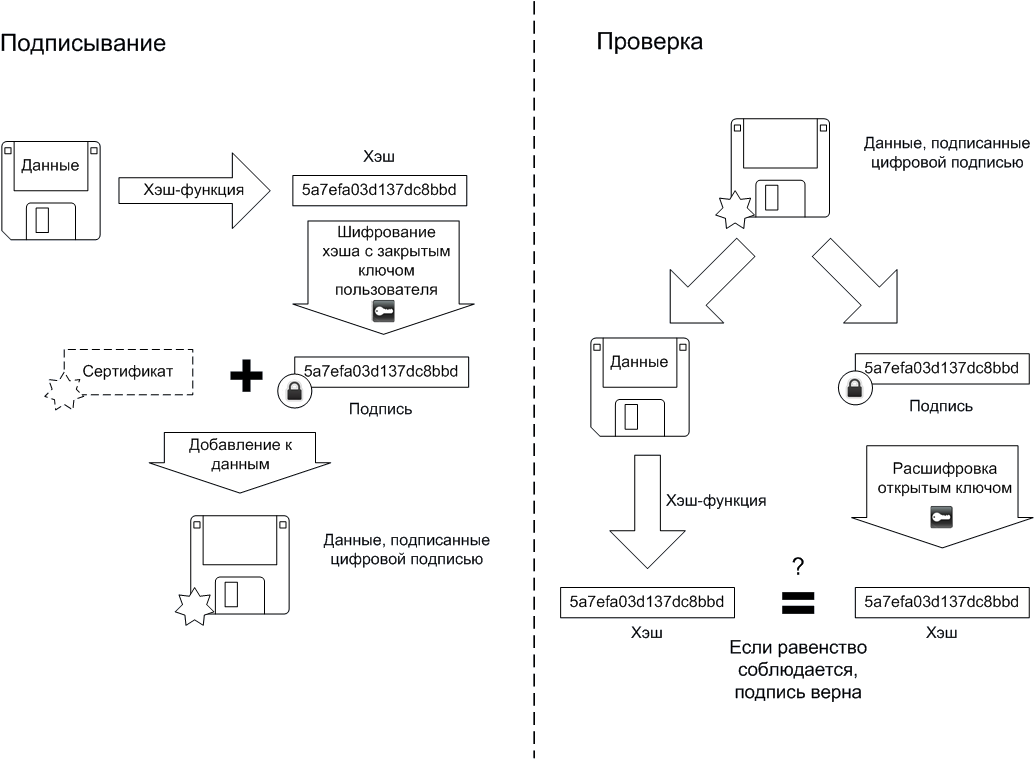
\includegraphics[width=0.9\linewidth]{CryptoSchema}
\caption[Цикл криптографичкеской цифровой подписи]{Схема, иллюстрирующая метод подписи и проверки ЭЦП Криптографические ЦП (КЦП) можно классифицировать по методам шифрования использующимся при их формировании на симметричные и ассиметричные.}
\label{fig:CryptoSchema}
\end{figure}
\subsubsection{ЦП на основе симметричных алгоритмах шифрования}
\par Симметричные схемы ЦП менее распространены чем асимметричные, так как после появления концепции цифровой подписи не удалось реализовать эффективные алгоритмы подписи, основанные на известных в то время симметричных шифрах. Первыми, кто обратил внимание на возможность симметричной схемы цифровой подписи, были основоположники самого понятия ЭП Диффи и Хеллман, которые опубликовали описание алгоритма подписи одного бита с помощью блочного шифра \cite{diffie1976}. Асимметричные схемы цифровой подписи опираются на вычислительно сложные задачи, например на разложение больших чисел на взаимно простые множители. Симметричные схемы основаны на хорошо изученных блочных шифрах. В связи с этим симметричные схемы имеют следующие преимущества:
\begin{itemize}
\item вычислительно менее затратны, по сравнению с аналогичными асимметричными шифрами;
\item возможно простого варьирования криптостойкости шифра;
\end{itemize}
\par Однако у симметричных ЭП есть и ряд недостатков:
\begin{itemize}
\item размер подписи сопоставим с размером подписываемого документа;
\item необходимость использования одноразовых ключей;
\end{itemize}
\subsubsection{ЦП на основе асимметричных алгоритмов шифрования}
\par Асимметричные схемы ЭП относятся к криптосистемам с открытым ключом. в данных схемах цифровой подписи подписание производится с применением закрытого ключа, а проверка подписи — с применением открытого. Схема асимметричного шифрования документа, представлена на \ref{fig:CryptoSchema}. Именно асимметричные схемы получили наибольшее распространение. Протоколы формирования ЦП сертифицированы, стандартизованы и имеют сформированную законодательную базу их применения \cite{gost34.10}. 
\par Общая схема цифровой подписи представленная в \cite{gost34.10} три процесса.
\begin{enumerate}
\item Генерация ключевой пары -- при помощи алгоритма генерации ключа, случайным образом выбирается закрытый ключ и вычисляется соответствующий ему открытый ключ.
\item Формирование подписи -- для заданного электронного документа с помощью закрытого ключа вычисляется подпись.
\item Проверка (верификация) подписи.
\end{enumerate}
\par Для того, чтобы использование цифровой подписи имело смысл, необходимо выполнение двух условий:
верификация подписи должна производиться открытым ключом, соответствующим именно тому закрытому ключу, который использовался при подписании; без обладания закрытым ключом должно быть вычислительно сложно создать легитимную цифровую подпись.















\subsection{Стеганографические ЭЦП}
\par Бурное развитие средств вычислительной техники в последнее десятилетие дало новый толчок развитию стеганографии. В отличие от криптографии, которая скрывает содержимое секретного сообщения, стеганография скрывает сам факт его существования. Стеганографию обычно используют совместно с методами криптографии, таким образом, дополняя её. 
\par Для защиты авторских прав мультимедийных файлов применяется создание и внедрение цифровых водяных знаков (ЦВЗ). ЦВЗ отличаются от криптографической ЭЦП тем, что информация «встроена» прямо в сигнал. Стеганографические цифровые водяные знаки невидимы, благодаря этому удается сохранить в тайне сам факт наличия метки, что служит дополнительным фактором защиты. 

\par Процесс формирования водяного знака может быть описан следующим образом. Сначала в сигнал-источник $S$ в доверенной среде внедряются водяные знаки при помощи функции $E$. В результате получается сигнал $S_E$. Следующий этап — распространение $S_E$ через сеть или любым другим способом. Во время распространения на сигнал может быть совершена атака. 
У получившегося сигнала $S_{EA}$ водяные знаки могут быть потенциально уничтожены или изменены. На следующем этапе функция обнаружения $D$ пытается обнаружить водяные знаки $\omega$. Отсутствие или повреждение водяного знака свидетельствует о подмене оригинального сигнала. А наличие неизменного знака $\omega$, подтверждает целостность полученных данных. Весь жизненный цикл цифрового водяного знака представлен на рисунке \ref{fig:DWMLifiCircle}.
\begin{figure}[h]
\centering
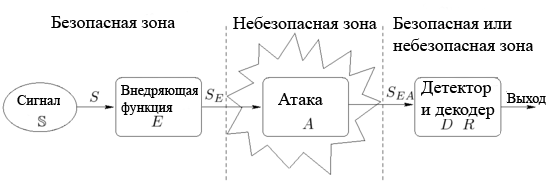
\includegraphics[width=0.9\linewidth]{./DWMLifiCircle}
\caption[Цикл стеганографической ЭЦП]{Цикл стеганографической ЭЦП \cite{lu2004}}
\label{fig:DWMLifiCircle}
\end{figure}

\par В работе \cite{gupta2015} представлена классификация ЦВЗ и подробный обзор методов их встраивания в исходные данные. Так по надежности выделяют следующие группы водяных знаков:
\begin{itemize}
\item \textit{чрупкие} -- нечитаемые, при малейшей модификации данных;
\item \textit{полу-хрупкие} -- выдерживаю незначительные изменения данных, но при вредоносном изменении становятся нечитаемыми, подобно хрупким;
\item \textit{надёжные}  -- противостоящие всем известным видам атак.
\end{itemize}
\par Методы нанесения ЦВЗ делятся на пространственные и частотные. 

 К пространственным методам относится метод \textit{LSB (Least Significant Bit)}.
Суть этого метода заключается в замене последних значащих битов в контейнере
 (изображения, аудио или видеозаписи) на биты скрываемого сообщения. Разница между пустым и заполненным контейнерами должна быть не ощутима
  для органов восприятия человека. Методы LSB являются неустойчивыми ко всем видам атак и могут быть использованы только при отсутствии шума в канале передачи данных.

Пример частотного метода нанесения ЦВЗ -- метод расширения спектра. Метод амплитудной модуляции, схожий с методом расширения спектра, также применяется для внедрения. Метод квантования не очень надёжен, но позволяет внедрить большой объём информации.
 Данные методы основываются на применении инвертируемых преобразованиях, таких как дискретное преобразование вейвлет или фурье, к несущему контейнеру. Добавление водяного знака осуществляется модификацией коэффициентов разложения (спектра) в соответствии с выбранным алгоритмом внедрения ЦВЗ. В завершении, применяется обратное преобразование для получение контейнера, содержащего ЦВЗ. Данные методы неравномерно распределяют встраиваемую информацию в несущий контейнер, делая задачу обнаружения и манипулирования с ЦВЗ сравнительно сложнее, по сравнению с пространственными методами встраивания. ЦВЗ, как правило, встраивается в средние частоты исходного сигнала, так как высокие частоты легко разрушаются операциями сжатия или масштабирвоания, а низкие частоты содержат основную воспринимаемую человеком информацию \cite{asatryan2009}. Это делает ЦВЗ, встроенный этими методами надежным или
  отличаются средней надёжностью, но очень маленьким информационной
   ёмкостью. 
   
   \par И частотные и пространственные методы имеют свои недостатки и особенности. Так недостатком частотных методов, может считаться высокая вычислительная сложность алгоритмов и малый объем встраиваемой информации, а пространственных относительная легкость обнаружения и ненадежностью. Поэтому в последнее время все больше внимание уделяется гибридизации данных методов, с целью получить заданные характеристики алгоритма встраивания и извлечения ЦВЗ. Так в работе \cite{deguillaume2003} исследователи представили гибридный метод, объединяющий свойства надежных и хрупких ЦВЗ. Надежный и хрупкий водяные знаки встраиваются в исходный сигнал последовательно. В работе \cite{al2007} исследователи поставили задачу улучшения производительности существующих методов. Для этого они разработали комбинированный подход на основе ДВП (дискретные вейвлет-преобразования) и ДКП (дискретное косинусное преобразование). В соответствии с данным подходом встраивание происходит на основе ДКП в двухуровневое ДВП от исходного сигнала (рисунок \ref{fig:HybridWM}).
   \begin{figure}[h]
\centering
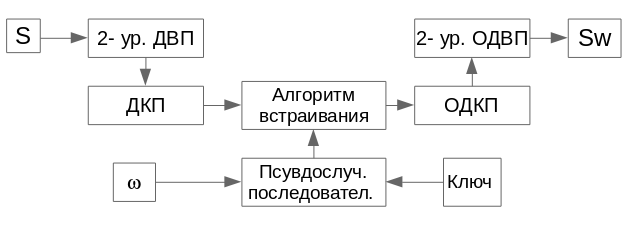
\includegraphics[width=0.7\linewidth]{./HybridWM}
\caption{Комбинирвоанная процедура формирования ЦВЗ.}
\label{fig:HybridWM}
\end{figure}

   




\subsubsection{Метод внедрения цифровой подписи в изображения}
\par В настоящее время предложено множество методов встраивания информации в изображение. Обзор методов встраивания ЦВЗ в изображения представлен в работе \cite{sagaydak2014}. Разработаны такие пространственные методы, как:
\begin{enumerate}
\item метод модификации младших бит \textit{LSB (Last Significant Bit)};
\item метод случайного интервала;
\item метод псевдослучайной перестановки (выбора);
\item метод блочного сокрытия.
\end{enumerate}
\par В отличие от метода LSB, в котором каждый бит
скрываемого сообщения записывается в последовательно идущие младшие биты, метод случайного интервала позволяет осуществлять случайное распределение битов этого сообщения по контейнеру, в результате чего расстояние между двумя встроенными
битами скрываемого сообщения определяется случайным образом. Но есть и недостаток данного метода -- биты скрываемого сообщения в контейнере
размещаются в той же последовательности, что и в
самом скрываемом сообщении. Поэтому, во избежание этого недостатка, прибегают к методу псевдослучайной перестановки (выбора), суть которого заключается в том, что при помощи генератора псевдослучайных чисел образуется последовательность индексов $j_1,j_2,\dots,j_k$ и выполняется сохранение $k$ -го бита
сообщения в пикселе с индексом $j_k$ .
Суть метода блочного скрытия заключается в следующем: изображение-оригинал разбивается на $l_m$
непересекающихся блоков $ \Delta i ( 1 \le i \le l_m ) $ произвольной конфигурации, для каждого из которых вычисляется бит чётности $b ( \Delta i ) = \sum_{j \in \Delta i}^{mod 2} LSB(C_j)$.
В каждом блоке выполняется скрытие одного секретного бита
$M_i$ . Если бит чётности $b ( \Delta i ) \ne M_i$ , то происходит
инвертирование одного из наименьших значащих битов блока $\Delta i$ , в результате чего $b ( \Delta i ) = M_i$ . Выбор блока может происходить псевдослучайно с использованием стеганоключа.

Также в своей работе Сагайдак Д. представил новый метод, позволяющий производить скрытое встраивание ЦВЗ как в изображение, так и физический документ. Идея метода встраивания основывается также на методе \textit{LSB}. 
Технически методика встраивания не меняется, но предложенный метод позволяет адаптировать ЦВЗ к конкретному документу, встраивая данные лишь в незначащие пиксели. Данный ЦВЗ относится к видимым. Но все же может применяться для подписи и удостоверения документа, если выполняется предположение о секретности ключа. Также в статье большое внимание уделено сложности легитимного распознавания наличия водяного знака и расшифровки информации содержащейся в нем. 
%Классификация методов стеганографической ЦП аудио файлов

\subsubsection{Метод внедрения цифровой подписи в аудио файлы}
\par  Методы встраивания ЦВЗ в аудио файлы можно классифицировать по области встраивания (\cite{borisova2015}) на
\begin{enumerate}
\item встраиваемые во временную область
		\begin{enumerate}
			\item метод замены наименьших значащих бит;
			\item метод внедрения информации с использованием эхо-сигнала;
			\item изменение масштаба временной (\textit{time base modulation});
		\end{enumerate}
\item встраиваемые в частотную область
		\begin{enumerate}
			\item Фазовое кодирование
			\item Растяжение спектра
			\item Модификация полосы частот
			\item Маскирование ЦВЗ
		\end{enumerate}
\end{enumerate} 
\par \textit{Метод замены наименьших значащих бит (НЗБ)} одинаково применяется к аудио файлам, как и к изображениям. Метод основывается на замене, в каждом значении амплитуды, наименьших значащих бит на биты сообщения. 
\par \textit{ Метод внедрения информации с использованием эхо-сигнала} Состоит в формировании звукового потока, состоящего из смеси нескольких идентичных сигналов, которые слегка отстают во времени. К параметрам эхо, несущим внедряемую
информацию, относятся: начальная амплитуда, время спада и сдвиг (время задержки между исходным сигналом и его эхо). Оригинальный сигнал смешивается с одной или несколькими точными копиями, которые слегка отстают во времени. Когда сдвиг
между оригинальным сигналом и его эхо уменьшается, ССЧ человека воспринимает эхо-сигнал как добавочный резонанс. Метод слабо устойчив к сжатию.
\par \textit {Метод фазового кодирования} предполагает встраивание информации в спектр исходного сигнала. Искомый сигнал с водяным знаком получается после обратного преобразования Фурье к модифицированному спектру.
 \par \textit {Метод растяжения спектра} добавляет псевдослучайная последовательность, представляющая собой «белый шум», модулируется сигналом несущей, представляющей ЦВЗ и затем добавляется к аудиосигналу-контейнеру.
 \par Метод \textit {изменения масштаба временной оси}  делит исходный сигнал на части, незначительно
 растягивая и сжимая  их. Местоположение и степень сжатия/растяжения являются величинами, которые используются для кодирования информации.
 
 \subsubsection{Цифровые отпечатки аудио файлов}
 \par Технология цифровых отпечатков используется в настоящее время
 для защиты различного рода информации, большей частью для защиты текстовых документов от утечек. Однако данная технология может быть распространена и на другие типы файлов, например на изображения, аудио- и видеофайлы. Она также является мощным средством удостоверения авторства на музыкальные произведение, так как процесс получения ЦО построен таким образом, что воспринимаемые одинаково звуковые образы, приводят к одинаковому отпечатку. Благодаря данному свойству, возможно определить идентичность музыкального фрагмента, перезаписанного без использования исходного файла (например, исполнение на музыкальном инструменте или с помощью синтезаторов звука).
 \par Два эффективных метода получения отпечатка файла рассмотрены в работе \cite{borisova2015}. Суть данных методов в сохранении спектральной характеристики сигнала для отдельных небольших его сегментов. Такой подход далек от совершенства, но хорошо подходит для отслеживания нелегального распространения контента в интернете, даже в сильно измененном виде.
 
 %встраивание в аудио файлы
\input{WMvideo.tex}
\subsection{Заключение}
\par \hspace{1.25cm}Почти сорок лет продолжается процесс развития методов формирования и проверки ЭЦП. За это время было предложено большое количество различных методов, но по-настоящему популярными стали лишь два протокола основанные на асимметричном шифровании. Криптографические ЭЦП имеют под собой как законодательную базу, так и большое количество программного обеспечения и накопленного опыта использования. Все это надежно закрепляет за данными методами место лидеров по распространению. 

\par Стеганографические методы цифровой подписи, вынуждены использовать методы шифрования для построения асимметричных схем ЦП. А значит, данные методы априори сложнее, требуют более сложных алгоритмов и сложнее программируются. Эти особенности сделали СЦП непопулярными. Хотя они и предоставляют дополнительный фактор защиты -- скрытность передачи. Последнее может в будущем стать негативным обстоятельством. В современном мире появилось дополнительное обстоятельство, которое может ограничить возможность использования скрытой передачи данных -- террористическая угроза. Криптографические методы не скрывают факта передачи защищенного сообщения, а значит поддаются контролю со стороны государственных специальных служб. В этой ситуации стеганографические методы передачи данных становятся объектом пристального внимания террористов.Также относительная редкость применения стеганографических методов, особенно в финансовой сфере,  обуславливает малую выгоду от разработки алгоритмов взлома и методов атак, делая потенциальные атаки слишком затратными. 
\par Последнее десятилетие на смену электронной коммерции приходит мобильная. Мобильные устройства отличаются малыми вычислительными мощностями. Этот фактор ограничивает уровень надежности алгоритмов шифрования, которые можно использовать для проведения электронных платежей. В данных условиях может стать целесообразным и экономически обоснованным разработка и поддержка уникального стеганографического метода шифрования и формирования ЦП для удостоверения платежей на мобильных устройствах. 
\par Надежность цифровой криптографической подписи основывается на математических  задачах, сложность которых настолько велика, что они не могут быть решены за время жизни самой подписи. У данного подхода есть две существенные проблемы. Во-первых, сложность этих задач не доказана, а значит надежность не гарантированная. Во-вторых, хоть и в очень отдаленной перспективе, производительность компьютеров может значительно возрасти с созданием рабочей версии квантового компьютера. Его возможности позволят решить все задачи, относящиеся к классу \textit{np}-полных за полиномиальное время. Это приведет к невозможности использовать традиционные асимметричные алгоритмы формирования ЦВЗ. Конечно, для решения этой проблемы были разработаны специальные квантовые алгоритмы цифровой подписи. В работе подробно рассмотрены алгоритмы КЦП электронных документов \cite{yin2015}. Но было бы интересно провести анализ гибридных крипто- стеганографических алгоритмов на стойкость к атаке с применением квантового компьютера.
\par  

\newpage
\printbibliography[env=gostbibliography,sorting=ntvy]



\end{document}